\documentclass[11pt,openany]{book}
% #1-Asignatura
% #2-Curso
% #3-Nombre
% #4-Link
% #5-Foto

\newcommand{\portada}[5]{
    \begin{titlepage}
        \begin{center}
            \vspace*{0.5cm}
            
            % Titulo con #1 lo mas grande posible
            {\Huge \textbf{#1}}

            
            \vspace{0.5cm}
            \LARGE
            Curso #2 
            
            \vspace{1cm}
            
            \Huge{\textbf{Grupo Viterbi}}

            \vspace{1cm}
            
\includegraphics[width=0.6\textwidth]{assets/Img/UGR-Logo.png}
            
            \vspace{0.5cm}

            \huge
            PRÁCTICA 5- PROGRAMACIÓN DINÁMICA
            
            \Large
            \vspace{1cm}
            \textbf{Integrantes:}  \\ 
             % Array con los nombres de los integrantes y el correo
             \begin{center}
                \begin{tabular}{c c }
                    \textbf{Miguel Ángel De la Vega Rodríguez} & miguevrod@correo.ugr.es \\
                    \textbf{Alberto De la Vera Sánchez} & joaquinrojo724@correo.ugr.es \\
                    \textbf{Joaquín Avilés De la Fuente} & adelaveras01@correo.ugr.es \\
                    \textbf{Manuel Gomez Rubio} & e.manuelgmez@go.ugr.es \\
                    \textbf{Pablo Linari Perez} & e.pablolinari@go.ugr.es
                \end{tabular}
             \end{center}
            \vspace{0.8cm}
            
            
            \large
             \vspace{1cm}
            Facultad de Ciencias UGR\\
            Escuela Técnica Ingeniería Informática UGR\\
            Granada\\
            #2 
            
        \end{center}
    \end{titlepage}
}



\usepackage{assets/formulas}
\usepackage[mathscr]{euscript}
\usepackage{bm}
\usepackage{float}
\hbadness=10000 % Suppress Underfull \hbox warnings

%========================================|Indice|===============================================%

\begin{document}
\portada{Algorítmica}{2023-2024}{Miguel Ángel De la Vega Rodríguez}{https://github.com/Miguevrgo/}{github.png}
\tableofcontents % Índice
\newpage %Salto de pagina tras el Indice


%======================================|Documento|==============================================%
\chapter{Autores}
\begin{itemize}
      \item \textbf{Miguel Ángel De la Vega Rodríguez:} 20\%
            \begin{itemize}
                  \item Algoritmos Greedy del Viajante
                  \item Redacción memoria sección Viajante
            \end{itemize}
      \item \textbf{Joaquín Avilés De la Fuente:} 20\%
            \begin{itemize}
                  \item Programacion Dijkstra
                  \item Programación creación de grafos (casos de prueba)
                  \item Redacción memoria sección Dijkstra
            \end{itemize}
      \item \textbf{Alberto De la Vera Sánchez: } 20\%
            \begin{itemize}
                  \item Redacción \LaTeX
                  \item Estudio de umbrales teóricos y empíricos de DyV
                  \item Graficas y ajustes
            \end{itemize}
      \item \textbf{Manuel Gomez Rubio} 20\%
            \begin{itemize}
                  \item Redacción y demostración del algorimo greedy
                  \item Redacción memoria del algoritmo Dijkstra
                  \item Programacion Dijkstra
            \end{itemize}
      \item \textbf{Pablo Linari Pérez:} 20\%
            \begin{itemize}
                  \item Programacion Aulas
                  \item Redacción Aulas
                  \item Redacción objetivos
            \end{itemize}
\end{itemize}

\chapter{Equipo de trabajo}

\begin{itemize}
      \item \textbf{Miguel Ángel De la Vega Rodríguez:} (Ordenador donde se ha realizado el computo)
            \begin{itemize}
                  \item AMD Ryzen 7 2700X 8-Core
                  \item 16 GB RAM DDR4 3200 MHz
                  \item NVIDIA GeForce GTX 1660 Ti
                  \item 1 TB SSD NvMe
                  \item Debian 12 Bookworm
                  \item Compilador GCC 12.2.0
            \end{itemize}
\end{itemize}

\chapter{Objetivos}

El objetivo de esta práctica es implementar la solución para cuatro problemas 
usando algoritmos Greedy. Los problemas a resolver son los siguientes: 
\begin{itemize}

      \item Hijo predilecto 
            Un individuo desea repartir sus N bienes entre sus dos hijos. Para cada bien se conoce el
            valor (positivo) del mismo. Previo al fallecimiento del individuo, el juzgado, de una forma ciega,
            determina un valor k, que nos indica el número de bienes que se le deben asignar a un hijo al
            otro se le asignan N - k. Conocido estos datos, el individuo desea distribuir los bienes entre
            sus hijos de forma que uno de ellos salga lo mas beneficiado posible. El beneficio obtenido por
            cada hijo se define como la suma de los beneficios de los bienes que se les lega.
      \item Asignación de aulas
            Se deben programar N exámenes en un día determinado, y para cada examen, el profesorado ha especificado el tiempo
            requerido para su realización y la hora de inicio ideal.
            El centro cuenta con m aulas disponibles, donde m es mayor que N , lo que garantiza la
            viabilidad de programar los exámenes. Sin embargo, cada vez que se utiliza un aula, el centro
            debe asegurar su vigilancia, lo que implica contratar a un vigilante distinto para cada aula
            utilizada.
      \item Problema del camino mínimo
            Tenemos un conjunto de n ciudades (puntos en un plano), cada una definida por las coor-
            denadas en el mapa $(x_i , y_i )$, con $i = 1, . . . , n$. Cada ciudad se puede conectar por carretera con
            un subconjunto de ciudades, asegurando que la red de vías que se genere crea un grafo conexo.
            Dada una ciudad de origen, x, y una ciudad de destino, y, se pide encontrar el camino de
            costo mínimo que permita viajar de x a y.
      \item problema del viajante de comercio
            Tenemos un conjunto de n ciudades (puntos en un plano), cada una definida por las coor-
            denadas en el mapa $(x_i , y_i )$, con $i = 1, . . . , n$. La distancia entre dos ciudades viene dada por la
            distancia euclídea entre sus coordenadas.El problema de viajante de comercio consiste en encontrar el orden en el que un viajante,
            partiendo de la ciudad de origen (por ejemplo $(x_1 , y_1 )$) pase por todas y cada una de las ciudades
            una única vez, para volver a la ciudad de partida, formando un ciclo.

\end{itemize}
Para cada uno de los problemas se ha de implementar
un algoritmoque de una solución óptima o aproximada dependiendo del problema. 
En todos los problemas se identificarán los componentes de un algoritmo Greedy y se demostrará que el algoritmo
greedy da la solución óptima en el caso de que el problema sea de optimización . 

Con esta práctica se pretende trabajar y comprender los algoritmos greedy y  reconocer las situaciones para las cuales puede 
ser beneficioso y usar esta técnica.

\chapter{Hijo predilecto}
En esta sección se abordará la resolución del primer problema a través de los algoritmos Greedy, siendo 
el enunciado del problema:

Un individuo desea repartir sus N bienes entre sus dos hijos. Para cada bien se conoce el
valor (positivo) del mismo. Previo al fallecimiento del individuo, el juzgado, de una forma ciega,
determina un valor k, que nos indica el número de bienes que se le deben asignar a un hijo (al
otro se le asignan N - k). Conocido estos datos, el individuo desea distribuir los bienes entre
sus hijos de forma que uno de ellos salga lo mas beneficiado posible. El beneficio obtenido por
cada hijo se define como la suma de los beneficios de los bienes que se les lega.

\section{Estructura de los datos}
\begin{enumerate}
      \item \textbf{Conjunto de candidatos}: El número de bienes del padre
      \item \textbf{Conjunto de seleccionados}:El vector del hijo1 (ya que hemos decidido
      que sea este hijo el que salga lo mas beneficiado posible)
      \item \textbf{Función solución}: Bucle for que recorre el vector padre, ya que hasta que no 
      se recorra el vector entero no se pueden haber reaprtido todos los bienes. 
      \item \textbf{Función de factibilidad}: En este caso siempre hay soluciones posibles
      \item \textbf{Función selección}:El conficional if/else que se encuentra dentro del primer bucle for que reparte
      la herencia entre el hijo1 y el hijo 2.
      \item \textbf{Función objetivo}: El hijo 1 que devuelve el return, ya que hemos decidido que
      que sea él el que obtenga el máximo beneficio posible
\end{enumerate}
\begin{lstlisting}

  pair<double,vector<double>> inheritance(vector<double> & father, vector<double> & son1, vector <double> & son2){
      //Conjunto candidato father
      //Conjunto de seleccionados son1
      int size=father.size();
  
      sort(father.begin(),father.end());
  
      srand(time(NULL));
      int partition=rand() % size;
  
      
      int range=(partition > (size-partition))? partition : (size-partition);
  
      int sum1=0;
      //Funcion solucion
      for (int i = 0; i<size;++i){
          
          //Funcion de seleccion
          if(i<range){
              son1.push_back(father.back());
              sum1+=father.back();
          }else{
              son2.push_back(father.back());
          }
          father.pop_back();
          
      }
      //Funcion objetivo
      return {sum1,son1};
  }
\end{lstlisting}

\section{Justificación}
Proposiciones:
\begin{enumerate}
      \item Definimos p(a) como el beneficio del bien a y $p(A)=\sum_{a \in A} p(a) $
      donde A es la herencia de un hijo
      \item Diremos que un conjunto A es solución cuando $p(A) \geq p(\overline{A})$ 
      siendo $p(\overline{A})$ la herencia del otro hijo 
      \item Diremos que un conjunto A de bienes es mejor solución que otro conjunto B cuando
      |A| = |B| y $p(A) \geq p(B)$ es solución
\end{enumerate}
Llamemos T al conjunto de los bienes de la herencia del padre y sea $B \subset T$ la herencia obtenida por el hijo
1(el que mejor beneficio va a obtener), generada por nuestro algorimo Greedy. B tendrá las 
siguientes propiedades:
\begin{equation*}
      p(B) \geq p(\overline{B}) \ \  \ \ \ \ , p(b_i) \geq p(\overline{b_j})  \  \ \ \ \ \ \ \forall i \in \{0,...,k\} \ \ \ \ \ \ \  \forall j \in \{k+1,n\}
\end{equation*}
Ahora para demostrar que B es una solución óptima vamos a proceder con reducción al absurdo.
Supongamos que B no es óptimo, entonces existe B' con |B'|=|B| y con $p(B') \geq p(B)$.
Elegimos $q \in \overline{B}$ con $ p(q) = max\ \ p(q')_{q' \in \overline{B}} $ 
y $s \in B$ con $ p(s) = min\ \ p(s')_{s' \in B } $ tal que  y los intercambiamos. Como B' es
una solución óptima, entonces, o todos los terminos de B' son mayores que los de B, o a partir de un 
número r en adelante $p(b')_{b'\in B'} > p(b)_{b \in B}$. Entonces al B no ser un solución óptima, al
haber intercambiado los elementos mencionados anteriormente, tendriamos que tener que $p(b')_{b'\in B'} > p(b)_{b \in B}$
a partir de un número r+1. Esto se debe a que, como trabajamo siempre con los mismos elementos,
al intercmbiarlos para llegar a la solución optima debe de estar en el conjunto B', demostrando que
B' es la solución óptima. Sin embargo, este resultado es una contradicción ya que al inercambiar los 
elementos de B y $\overline{B}$ como $p(b_i) \geq p(\overline{b_j})$, lo demostrado anteriormente es falso.
\section{Estudio teórico y empírico}
En cuanto al estudio teórico podemos ver a simple vista que el codigo tiene una eficiencia O(n), debido al bucle
for de las líneas 17-28. A continuación mostraremos como el estudio empírico verifica dichos datos. Para el estudio 
empírico hemos usado vectores iniciales, es decir, la herencia del padre, iniciando con tamaño 1000 hasta 100000 
incrementando en 1000 el tamaño del vector en cada ciclo.

\begin{figure}[H]
      \centering
      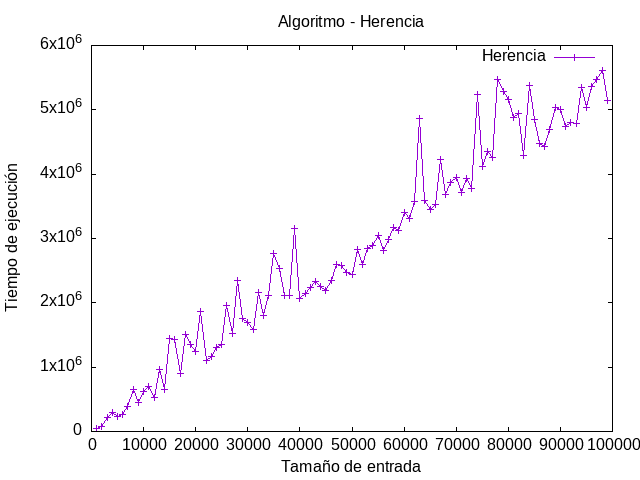
\includegraphics[width=0.6\linewidth]{assets/Img/Herencia.png}
      \caption{Herencia}
      \label{fig:Herencia}
\end{figure}

\chapter{Asignación de aulas}
En esta sección se estudia lo referente al algoritmo usado para resolver el segundo 
problema el cual nos pide lo siguiente :

Se quieren ralizar N exámenes en un día en la ETSIIT , el centro cuenta con m aulas donde m es mayor
que N . Sin embargo cada vez que se utiliza un aula el centro debe contratar un vigilante por tanto 
se debe diseñar un algoritmo que clacule en base al horario de los exámenes el menor costo posible 
para la escuela , es decir hay que encontrar la manera de distribuir los exámenes para usar el menor número
de aulas posibles .

\section{Estructura de los datos}
Una vez planteado el problema porcedemos a describir las herramientas que hemos usado para resolverlo 
Para representar los horarios de los exámenes hemos usado la siguiente estructura :

\begin{lstlisting}
      struct tiempo{
            int hora;
            int min;
            tiempo(int h , int m){
                hora = h;
                min = m ;
            }
      };
      struct examen{
            tiempo inicio; // Hora de inicio
            tiempo final; // Hora de finalizacion
            examen(tiempo t , tiempo t1) : inicio(t), final(t1){}
      };
        
      struct compare{
            bool operator()(const examen&a,const examen&b){
                if(a.inicio.hora==b.inicio.hora){
                    return a.inicio.min < b.inicio.min;
                }
                return a.inicio.hora < b.inicio.hora;
            }
      };
        
\end{lstlisting}

El struct compare se utiliza para ordenar el vector de entrada de exámenes de manera que se ordenen
de menor a mayor en función de la hora de inicio de los exámenes , de esta manera se facilita la
ejecución del algoritmo que se encarga de asignar los exámenes a las aulas de la manera más eficiente
posible.

\section{Algoritmo}

A continuación vemos el algoritmo usado para la distribución de las aulas.

\begin{lstlisting}[language=C++]
      bool sesolapan(examen e1,examen e2){
            if(e1.final.hora == e2.inicio.hora){
                return e1.final.min >e2.inicio.min;
            }
            return e1.final.hora > e2.inicio.hora;
        }
        
        int minAulas(const vector<examen> & v){
        
            // Conjunto de candidatos v
        
            int naulas = 1;
            vector<queue<examen>> horario;
            //Conjunto de seleccionados horario (vector de colas , cada cola es un aula)
            
            horario.emplace_back(queue<examen>());
            horario[0].push(v[0]);
            int i;
            //
            for(int nex = 1;nex < v.size();nex++){
                i=0;
                //Funcion de seleccion
                while(i<horario.size() && (sesolapan(horario[i].back(),v[nex]))){i++;}
                //Funcion de factibilidad
                if(i==horario.size()){
                    horario.emplace_back(queue<examen>());
                    horario[i].push(v[nex]);
                    naulas++;
                }
                else{
                    horario[i].push(v[nex]);
                }
            }
            return naulas; //Funcion objetivo 
      }
\end{lstlisting}

Uno de los factores importantes que hay que destacar de este algoritmo es que el vector \textbf{v} se supone 
ordenado de mayor a menor , es decir que en el vector los exámenes aparecen en orden creciente de 
horario de inicio de esta manera la asignación de aulas es más rápida y eficiente.

El algoritmo comienza añadiendo el primer examen al primer aula , cada aula se representa con una posición del vector 
y el horarario del aula se representa con una cola ya que solo nos interesa el último examen hecho en el aula.

Posteriormente se entra al bucle for el cual recorre todo el vector de candidatos ya que todos los exámenes deben
ser realizados . 

Dentro del bucle for se entra a un while el cual comprueba mediante la función \textbf{sesolapan(examen e1 ,examen e2)}
si el examen que está buscando un aula se solapa con el que se está realizando en el aula , si no se solapan se añade a 
ese aula , si se solapan se busca otra aula en la que no se solapen y se añade a esa aula. En el caso de que se hallan agotado
las aulas actuales se crea una nueva aula y se añade el examen a esa aula.

\section{Justificación Greedy}

En este apartado vamos a analizar el algoritmo identificando los componentes que lo hacen un algoritmo greedy 
y demostrando que siempre llega a la solución óptima.
\section{Componentes}
\begin{itemize}
      \item Candidatos a seleccionar:\\
            En este problema los candidatos a seleccionar son los exámenes 
            los cuales se tendrán que distribuir entre aulas.
      \item Candidatos seleccionados:
            Los candidatos seleccionados en este caso son el conjunto aula-exámenes
            del cual nos interesa para la solución el número de aulas en el que se distribuyen los exámenes.

      \item Función Solución:
            La función silución en este caso es el for de la linea 20
            ya que la solución se alcanza cuando el vector de 
            exámenes se ha conseguido recorrer entero , lo que significará que 
            todos los exámenes han sido asignados a un aula.
            Esto siempre se conseguirá dada la condición del problema.
            

      \item Función de Selección:\\ 
            La función de selección en este algoritmo se encuentra
            en las líneas 21 a 24 donde el bucle while recorre las 
            posibles aulas para seleccionar la primera en la que haya 
            un hueco para el posible candidato .

      \item Función de factibilidad:\\
            
            % La función de factibilidad se encuentra entre las líneas 24 y 32 
            % la cual consiste de una estructura if-else que comprueba si se necesita 
            % crear una aula nueva o se puede añadir a un aula ya existente.
            
            % En este caso siempre es posible completar un conjunto de candidatos para 
            % dar la solución al problema ya que el numero de aulas es mayor que el de exámenes.

            En este caso no hay función de factibilidad ya que siempre se puede seleccionar un exámen por la 
            condición inicial del problema .


      \item Funcion objetivo: \\
            La función objetivo es la línea 34 en la cual se devuelve la cantidad de aulas usadas.

\end{itemize}

\subsection{Demostración }
Una vez definidas las funciones, conjuntos de candidatos, etc,  pasaremos a realizar la demostración del algortimo greedy.
Para la demostración se usará el método de inducción en el cual definiremos dos casos base uno para 1 exámen y otro para 2 
exámenes para que sea más facil la  demostración.

\begin{itemize}
      \item Caso base n=1:
            En el caso base se tiene un solo examen y por tanto solo se necesita un aula para realizarlo.Por lo que se 
            asigna el aula y el examen sin problema
      \item Caso base n=2:
            En el caso base n=2 se tienen dos exámenes y caben 2 posibilidades, que los exámenes se solapen por tanto 
            se necesitarán 2 aulas o que no se solapen y por tanto se necesitará solo un aula.

      \item Hipótesis de inducción:
            Supongamos que el algoritmo es óptimo para n exámenes y veamos que también lo es par n+1 exámenes.
      \item Paso de inducción:
            Supongamos que para n exámenes tenemos una solución óptima de k aulas . Veamos que ocurre para n+1 
            donde caben dos opciones :
            \begin{itemize}
                  \item Que el exámen n+1 se solape con alguno de los n exámenes anteriores  que se están realizando en una 
                        de las k aulas por tanto se necesitará una nueva aula para el examen n+1 por lo que el número de aulas aumentará a 
                        k+1 y como la solución para n exámenes era óptima la solución para n+1 exámenes también lo será ya que el único cambio
                        es el de aniñdir un aula. 
                  \item Que el examen n+1 no se solape con ninguno de los n exámenes anteriores , en este caso se podrá 
                        añadir a un aula ya existente en la que no se esté haciendo ningún exámen 
                        por lo que el número de aulas necesarias será k y como para n exámenes k era la solución óptima y este último 
                        exámen no ha modificado el valor de k la solución para n+1 exámenes también será óptima.
            \end{itemize}
      \item Conclusión:
            Dado que se ha demostrado que existe solución óptima para n+1 exámenes concluimos 
            la demostración por inducción.

\end{itemize}
\section{Ejecución del Algoritmo}
Para ejecutar el programa se usan los siguientes parámetros:
./Aulas <número de exámenes> <duración máxima del examen>

0:37 - 2:16 
0:51 - 1:56 
2:44 - 5:11 
8:32 - 10:2 
10:47 - 11:17 
13:12 - 16:12 
13:45 - 13:56 
15:51 - 17:10 
17:51 - 20:46 
18:30 - 18:30 
19:24 - 19:43 
19:51 - 22:34 
21:51 - 23:57 
22:18 - 23:36 \\

------------------------------\\

0\\
0:37 - 2:16   \\            
2:44 - 5:11 \\
8:32 - 10:2 \\
10:47 - 11:17 \\
13:12 - 16:12 \\
17:51 - 20:46 \\
21:51 - 23:57 \\

1\\
0:51 - 1:56 \\
13:45 - 13:56 \\
15:51 - 17:10 \\
18:30 - 18:30 \\
19:24 - 19:43 \\
19:51 - 22:34 \\

2 \\
22:18 - 23:36 

numero de aulas : 3

\section{Análisis Teórico}
Comenzamos mirando el interior del bucle for donde la eficiencia entre 
las líneas 25 y 32 donde la cual es de $O(1)$ y por tanto tiene un tiempo 
de ejecución constante el cual llamaremos a . 
En la línea 21 el bucle while se ejecuta cuando las aulas se solapen 
por tanto en el peor caso si se solapan todas las aulas recorrerá el vector horario 
horario.size()-1 veces por tanto la eficiencia de este bucle es de $O(n)$ 
el bucle for v.size()-1-1 veces por tanto la eficiencia de este bucle es de $O(n)$
y al estar el bucle while dentro del for la eficiencia quedaría como 

\begin{equation*}
      \sum_{i=1}^{v.size -2} \sum_{i=0}^{horario.size -1}  a
\end{equation*}

Tomamos el peor de los casos donde todas las aulas se solapen 
por tanto v.size = horario.size y si sustituimos por n tenemos que:
\begin{equation*}
      \sum_{i=1}^{n -2} \sum_{i=0}^{n-1}  a = \sum_{i=1}^{n -2} na = n\cdot a \sum_{i=1}^{n -2} 1 = n\cdot a \cdot (n-2) = an^2 -2an
\end{equation*}
Por tanto el Alogritmo tiene eficiencia de $O(n^2)$

\section{Análisis empírico}
Para el análisis empírico se ha usado un generador de horarios 
aleatorios y como tamaño de datos se han usado de 5000 a 125000
exámenes incrementando en 5000 exámenes cada test .

\begin{figure}[H]
      \centering
      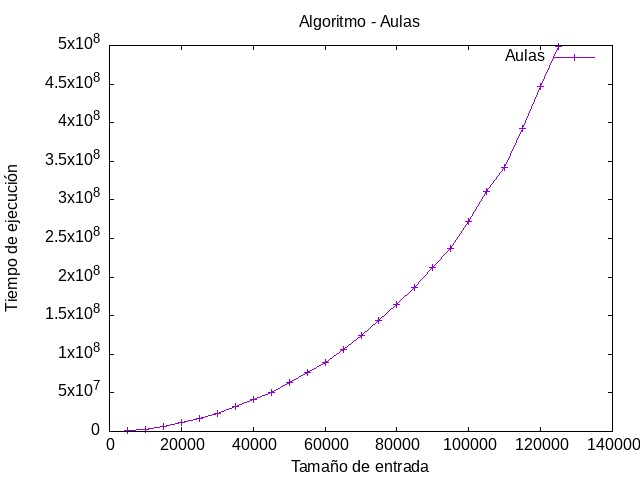
\includegraphics[width=0.8\textwidth]{assets/Img/Aulas.png}
      \caption{Ejecución de 5000 a 125000 examenes de maximo 3 horas}
\end{figure}


\chapter{Camino mínimo} % Manuel y Joaquin
En esta sección se analiza todo lo relacionado con el tercer problema propuesto, el problema del camino mínimo entre dos ciudades. 
Comentaremos el algoritmo usado, es decir, el \textbf{algoritmo de Dijkstra}, y su implementación en C++, así como la justificación de su uso mediante
la demostración de que dicho algoritmo Greedy calcula la solución óptima.  \\
Destacar también que mostraremos la gestión que hemos hecho para la creación de los posibles casos (\textbf{grafos}), así como la 
ejecución de los mismos y la obtención de los resultados.

\section{Algoritmo de Dijkstra}
A continuación, veremos las distintas partes usadas para la demostración como bien pueden ser la función de selección o
la forma en que se seleccionan los nodos, y finalmente la demostración mediante inducción. \\
Definiremos pues cada parte del algoritmo: \\
\begin{itemize}
      \item Candidatos a seleccionar:\\
            En este problema los candidatos a seleccionar son los diferentes vértices del grafo que no hayan sido \\
            seleccionados previamente.
      \item Candidatos seleccionados:
            Llamaremos $\mathscr{S}$ al conjunto de los vértices seleccionados. \\
            En nuestro problema siempre partiremos de un vértice, por lo que, como mínimo siempre habrá un vértice en $\mathscr{S}$ que será el origen 
            desde donde partiremos a considerar los nuevos vértices.

            Una vez definido $\mathscr{S}$ hay que definir también $\mathscr{V}\setminus\mathscr{S}$ que será el conjunto de vértices candidatos a ser seleccionados,
            siendo por tanto, $\mathscr{V}$ el total de vértices del grafo.

      \item Función Solución:\\
            La solución se obtendrá cuando el nodo origen y el destino estén en $\mathscr{S}$, siendo el nodo destino el último seleccionado, teniendo así el camino mínimo $\mathscr{M}(o,v)$

      \item Función de Selección:\\ 
            La función de selección en este algoritmo es siempre tomar el camino de menor distancia posible entre los nodos que estén conectados con el origen, actualizando los nuevos posibles candidatos 
            tras una elección

      \item Función de factibilidad:\\
            Un vértice es seleccionable en el caso en el que su distancia respecto al origen no sea infinito, esto quiere decir que debe haber vérices dentro de los seleccionados que nos permitan, mediante
            caminos directos, alcanzar el vértice sobre el que nos preguntamos si es factible

      \item Funcion objetivo: \\
            El problema tendrá siempre tamaño $\mathscr{V}$, es decir, el número de vértice del grafo. (Se puede considerar el tamaño real como $\mathscr{V}-1$ ya que el nodo de origen siempre es el primero en seleccionarse sin
            tener en cuenta ningún criterio)
\end{itemize}
Una vez definidas las funciones, conjuntos de candidatos, etc,  pasaremos a realizar la demostración del algortimo greedy.

\subsection{Demostracion de la optimalidad del algoritmo de Dijkstra}
Para la demostración, usaremos inducción y reducción al absurdo, veámoslo paso a paso:
\begin{itemize}
      \item El caso base será cuando \#$\mathscr{S}=1$ o bien es igual a 2.\\
            En ambos casos el algorimo nos dará una solución trivial, ya que, en el caso \#$\mathscr{S}=1$ la distancia mínima entre un vértice consigo mismo es 0.
            En el caso de que \#$\mathscr{S}=2$, tenemos que la distancia mínima entre los dos nodos será la que los conecte con menor distancia, puesto que el grafo es conexo y no pueden no estar conectados.
      \item Paso de inducción:
            Sea $v$ el nuevo vértice que ha sido seleccionado por el algoritmo, y por tanto $v\in \mathscr{S}$.\\
            Ahora usaremos reducción al absurdo y tomaremos que la distancia $d(v)$ (que representa algún camino de $o$ a $v$, con $o$ como el nodo de origen) no es la longitud mínima.\\
            Tomaremos entonces, $\mathscr{L}$ como la distancia mínima de $o$ a $v$. Y tenemos en cuenta que en $\mathscr{L}$ hay un camino que parte de un nodo x, ($c(x,y)$ camino de x a y), siendo x el último nodo en $\mathscr{S}$\\
            Con todo esto tenemos:
            \begin{equation*}
                  \mathbf{d(v)}\bm{>}\mathscr{M}(o,v)=\mathscr{M}(o,x)+c(x,y)+\mathscr{M}(y,v) > \mathscr{M}(o,x)+c(x,y)= d(x)+c(x,y)\geq\mathbf{d(y)}
            \end{equation*}
            Donde hemos usado que $\mathscr{L}$ es el camino mínimo y está formado por la primera igualdad.\\
            En la primera desigualdad, usamos la hipótesis, puesto que suponíamos que $d(v)>\mathscr{L}$, mientras que en la última igualdad
            se usa la hipótesis de inducción, pues $d(x)=\mathscr{M}(o,x)$ es la distancia mínima de $o$ a $x$, ya que es un punto escogido con anterioridad, y por tanto, $x\in \mathscr{S}$\\
            Por último, nos falta explicar la contradicción que hemos obtenido, que está marcada en negrita.
            Esta contradicción nos indica que al ser la distancia de y menor que la de v, nuestro algoritmo debería haber elegido al vétice $y$ en vez de a $v$\\
            Luego, hemos probado la optimalidad de nuestro algoritmo.

\end{itemize}

\section{Estructura de datos y grafos}
Para la implementación del algoritmo de Dijkstra, hemos usado una estructura de datos que nos permita representar un grafo, en este caso,
hemos usado una matriz de adyacencia. Por tanto, a continación se explicara de forma detallada la creación de dichos grafos así como la forma de 
representarlos en archivos de texto, ya que al ser la primera vez que se trabaja con grafos es útil tener
claro como se ha hecho. \\ \\
Para la creación de los grafos se ha hecho uso de un programa en C++ que nos permite generar grafos aleatorios, a partir
de un vector que tenga los distintos puntos. Destacar en primer lugar, que para la creación de los puntos de forma aletoria hemos usado 
de este trozo de código:
\begin{lstlisting}[language=C++]
// Inicializar el generador de numeros aleatorios
srand(time(NULL));

// Generar puntos aleatorios y escribirlos en el archivo
for (int i = 0; i < numPuntos; i++) {
      int coordX = rand() % (rangoMax + 1); // Generar coordenada x
      int coordY = rand() % (rangoMax + 1); // Generar coordenada y
      file << coordX << " " << coordY << endl; // Escribir coordenadas al archivo
}
\end{lstlisting}
donde file es el archivo donde se escriben los puntos, numPuntos es el número de puntos que se quieren generar y rangoMax es el rango
máximo de las coordenadas. \\
Tenemos ahora archivos con distintos puntos aleatorios, y para la creación de los grafos, hemos usado las siguientes dos funciones:
\begin{lstlisting}[language=C++]
// Funcion para la creacion de grafos a partir de un vector de puntos en 2D
void creacionGrafos(const vector<Point>& vec, vector<vector<double>>& matriz) {
      int size = vec.size();
      
      // Inicializacion de srand con resolucion mas alta
      unsigned seed = chrono::high_resolution_clock::now().time_since_epoch().count();
      srand(seed);
      
      for (int i = 0; i < size; i++) {
            // Num nodos que conectaremos con el nodo i
            int conexiones = rand() % (size/3 - 1) + 1; // Asegura al menos una conexion por nodo
            for (int j = 0; j < conexiones; j++) {
                  int nodo_conectar;
                  do {
                  nodo_conectar = rand() % size;
                  } while (nodo_conectar == i); // Asegura no conectarse a si mismo
      
                  // Aniadimos su distancia a la matriz de forma simetrica
                  double distancia = vec[i].distanceTo(vec[nodo_conectar]);
                  matriz[i][nodo_conectar] = distancia;
                  matriz[nodo_conectar][i] = distancia; // Simetria
            }
      }
      
      // Garantizar que al menos un nodo (p_inicio) este conectado a todos los demas
      int p_inicio = rand() % size;
      for (int i = 0; i < size; i++) {
            if (i != p_inicio) {
                  double distancia = vec[p_inicio].distanceTo(vec[i]);
                  matriz[p_inicio][i] = distancia;
                  matriz[i][p_inicio] = distancia; // Simetria
            }
            matriz[i][i] = 0; // Distancia a si mismo es cero
      }
}

// Funcion para la creacion de grafos a partir de un vector de puntos en 2D
void creacionGrafos2(const vector<Point>& vec, vector<vector<double>>& matriz) {
    int size = vec.size();
    vector<Point> conectados(size);
    vector<Point> noConectados=vec;

    // Inicializacion de srand con resolucion mas alta
    unsigned seed = chrono::high_resolution_clock::now().time_since_epoch().count();
    srand(seed);

    int nodo_inicial=rand()%noConectados.size();
    conectados[0]=noConectados[nodo_inicial];
    // Eliminados dicho nodo
    noConectados.erase(noConectados.begin()+nodo_inicial);

    for(int i=1; i<size; i++){
        int nodo_conectar=rand()%noConectados.size();
        int nodo_conectado= rand()%conectados.size();
        matriz[nodo_conectado][nodo_conectar]=vec[nodo_conectado].distanceTo(vec[nodo_conectar]);
        matriz[nodo_conectar][nodo_conectado]=vec[nodo_conectado].distanceTo(vec[nodo_conectar]); // Parte simetrica
        conectados[i]=noConectados[nodo_conectar];
        noConectados.erase(noConectados.begin()+nodo_conectar);
    }

    for (int i = 0; i < size; i++) {
        // Num nodos que conectaremos con el nodo i
        int conexiones = rand() % (size/3 - 1) + 1; // Asegura al menos una conexion por nodo
        for (int j = 0; j < conexiones; j++) {
            int nodo_conectar;
            do {
                nodo_conectar = rand() % size;
            } while (nodo_conectar == i); // Asegura no conectarse a si mismo

            // Aniadimos su distancia a la matriz de forma simetrica
            double distancia = vec[i].distanceTo(vec[nodo_conectar]);
            matriz[i][nodo_conectar] = distancia;
            matriz[nodo_conectar][i] = distancia; // Simetria
        }
    }
}
\end{lstlisting}
donde la matriz pasada por referencia será la llamada \textbf{matriz de adyacencia} que representa el grafo, y \textbf{vec} es el vector de puntos
leido del archivo. Importante recalcar las líneas donde se implementan las distancias de forma simétrica en la matriz.\\ 
Hemos usado dos funciones para la creación de los grafos, una que conecta un nodo con todos los demás (\textbf{creacinoGrafos}) y otra que conecta los nodos de forma aleatoria 
(\textbf{creacionGrafos2}).\\ \\
Las matrices de adyacencia que hemos obtenido, las hemos guardado en archivos de texto, para poder leerlas posteriormente y ejecutar
el algoritmo de Dijkstra sobre ellas, por lo que para ello hemos creado funciones que permitan leer y guardar dichas matrices, pues hay que recordar que 
los puntos que no tengan conexión directa, tendrán un valor de infinito en la matriz. Tenemos así estas dos funciones, una para 
escribir la matriz en un archivo de texto y otra para leerla:
\begin{lstlisting}

// Funcion para mostrar una matriz en un archivo de salida
void mostrarMatriz(ofstream &salida, const vector<vector<double>>& matriz) {
      int anchoMaximo = 0;
      const string infStr = "INF";

      // Primero, vamos a calcular el ancho maximo para los numeros y "INF"
      for (const auto& fila : matriz) {
            for (double elemento : fila) {
            ostringstream ss;
            if (elemento != numeric_limits<double>::max()) {
                  ss << fixed << setprecision(3) << elemento; // Convertir el numero a string con 3 decimales
            } else {
                  ss << infStr; // Si es infinito, usamos "INF"
            }
            anchoMaximo = max(anchoMaximo, static_cast<int>(ss.str().length())); // Actualizar el ancho maximo
            }
      }

      // Configuracion de la salida con el ancho encontrado
      salida << fixed << setprecision(3);

      // Mostrar la matriz con el ancho maximo
      for (const auto& fila : matriz) {
            for (double elemento : fila) {
            if (elemento == numeric_limits<double>::max()) {
                  salida << right << setw(anchoMaximo) << infStr << "\t";
            } else {
                  salida << right << setw(anchoMaximo) << elemento << "\t";
            }
            }
            salida << endl;
      }
}
      
// Funcion para leer la matriz desde un archivo
void lecturaMatriz(ifstream &leer, vector<vector<double>>& matrix) {
      string line;
      while (getline(leer, line)) {
            vector<double> row;
            stringstream ss(line);
            string val_str;
            while (ss >> val_str) {
            if (val_str == "INF") {
                  row.push_back(numeric_limits<double>::max());
            } else {
                  row.push_back(stod(val_str));
            }
            }
            matrix.push_back(row);
      }
}
\end{lstlisting}
donde \textbf{numeric\_limits<double>::max()} es el valor que hemos usado para representar la ausencia de conexión entre dos nodos, que
en la matriz escrita y leida se mostrará como \textbf{INF} de infinito.\\ \\
\section{Estudio eficiencia teórica}
En esta sección estudiaremos la eficiencia teórica de dicho algorimto, para ello veamos primero el código usado:
\begin{lstlisting}
// Funcion auxiliar para encontrar el vertice con la distancia minima
int minDistance(const vector<double>& dist, const vector<bool>& visited) {
      double min = INF;
      int min_index = -1; // Inicializado a -1 para detectar errores si no se encuentra ninguno

      for (int v = 0; v < dist.size(); v++) {
            if (!visited[v] && dist[v] <= min) {
                  min = dist[v];
                  min_index = v;
            }
      }
      return min_index;
}
// Funcion para implementar el algoritmo de Dijkstra desde inicio hasta un nodo destino w
void dijkstra(const vector<vector<double>>& graph, int inicio, int final) {
      int V = graph.size();
      vector<double> dist(V, INF); // Distancias minimas
      vector<bool> visited(V, false); // Nodos visitados
      vector<int> parent(V, -1); // Para rastrear el camino

      // Inicializar la distancia del nodo inicial a si mismo como 0
      dist[inicio] = 0;
      
      for (int count = 0; count < V - 1; count++) {
            int u = minDistance(dist, visited);
            visited[u] = true;

            // Si el nodo seleccionado es el nodo destino, terminar el algoritmo
            if (u == final)
            break;

            for (int v = 0; v < V; v++) {
                  if (!visited[v] && graph[u][v] != 0 && dist[u] != INF && dist[u] + graph[u][v] < dist[v]) {
                        dist[v] = dist[u] + graph[u][v];
                        parent[v] = u; // Registrar el nodo padre para rastrear el camino
                  }
            }
      }
      
      // Imprimir la distancia minima
      cout << "Distancia minima desde el nodo " << inicio << " al nodo " << final << ": " << dist[final] << endl;

      // Imprimir el camino recorrido
      printPath(parent, inicio, final);
}
       
\end{lstlisting}
donde hemos definido \textbf{const double INF = numeric\_limits<double>::max()} para representar la ausencia de conexión entre dos nodos.
La función \textbf{minDistance} nos permite encontrar el nodo con la distancia mínima, y la función \textbf{dijkstra} nos permite ejecutar
el algoritmo de Dijkstra desde un nodo inicial hasta un nodo final, mostrando la distancia mínima y el camino recorrido, haciendo uso
de la función \textbf{printPath} que se muestra a continuación:
\begin{lstlisting}
// Funcion para imprimir el camino recorrido
void printPath(const vector<int>& parent, int src, int dst) {
      stack<int> path;
      int current = dst;
      while (current != src) {
            path.push(current);
            current = parent[current];
      }
      path.push(src);

      cout << "Camino desde el nodo " << src << " al nodo " << dst << ": ";
      while (!path.empty()) {
            cout << path.top() << " ";
            path.pop();
      }
      cout << endl;
}
\end{lstlisting}
Visto el código, pasamos a analizar la eficiencia teórica del algoritmo de Dijkstra.\\ \\
Para ello, primero veamos que la función \textbf{minDistance} tiene una eficiencia de $O(V)$, donde $V$ es el número de vértices del grafo, es decir, tomando $V=n$
como el tamaño del problema, tenemos por tanto que la eficiencia de dicha función es $O(n)$. \\ \\
Por otro lado, en la función \textbf{dijkstra} desde la línea 16 hasta la línea 19 se inicializan varios vectores con valores
predeterminados y con tamaño $V=n$ (número de filas, es decir, la cantidad de puntos), por lo que la eficiencia de esta parte es $O(n)$. Es importante recalcar que aunque se tome 
$V=graph.size()$, en realidad, $V$ es el número de vértices del grafo, ya que para cada fila de la matriz de adyacencia tenemos las distintas distancias con el resto de nodos. \\
A continuación, encontramos un bucle que se ejecuta $V-1$ veces, y en cada iteración se llama a la función \textbf{minDistance}, por lo que la eficiencia de este bucle es $O(n^2)$. De hecho
en cada iteración del bucle de la línea 24 se hace otro bucle que se ejecuta $V$ veces (línea 32), para actualizar las distancias a los nuevos nodos, por lo que tomando la función suma, tenemos que la eficiencia de este bucle
es $O(n^2)$.\\
Por último, la llamada a la función \textbf{printPath} tiene una eficiencia de $O(n)$, ya que se recorre (imprimiento) el camino recorrido, que como mucho tendrá $n$ nodos.\\ \\
Por tanto, la eficiencia teórica del algoritmo Dijkstra implementado es $O(n^2)$, donde $n$ es el número de nodos del grafo.\\ \\
\section{Representaciones gráficas}
Finalmente, mostraremos varios ejemplos de la ejecución del algoritmo de Dijkstra sobre distintos grafos, y la representación gráfica de los mismos
 donde se pueden observar los posibles caminos y el mínimo escogido por dicho algoritmo.\\ \\
Veamos a continuación un ejemplo en el que se han graficado 7 puntos con distintas conexiones y se ha elegido un camino:
\begin{figure}[H]
      \centering
      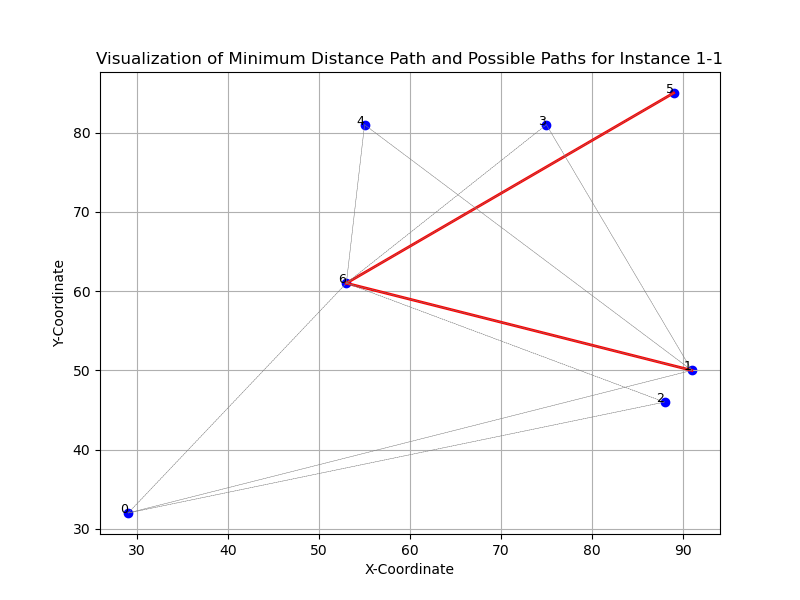
\includegraphics[width=0.8\textwidth]{assets/Img/GraficaCaminoMinimo-1-1.png}
      \caption{Grafo con 7 puntos y conexiones}
\end{figure}
Mostremos a continuación otro gráfico con los mismos puntos y distintas conexinoes y veamos como cambia el camino
mínimo escogido:
\begin{figure}[H]
      \centering
      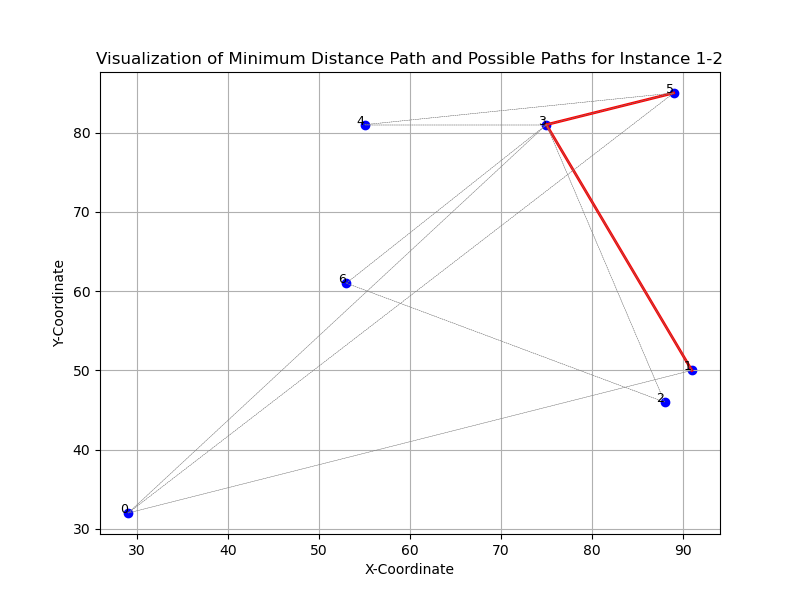
\includegraphics[width=0.8\textwidth]{assets/Img/GraficaCaminoMinimo-1-2.png}
      \caption{Grafo con 7 puntos y conexiones}
\end{figure}
Destacar que en ambos casos se busca el camino mínimo entre el nodo 1 y 5.\\ \\
También podemos observar casos donde si exite un camino directo entre los nodos inicial y final, el algoritmo escogerá dicho
camino mínimo como es de esperar, veámoslo
% Se muestran dos gráficos en paralelo
\begin{figure}[H]
      \centering
      \begin{minipage}{0.49\textwidth}
            \centering
            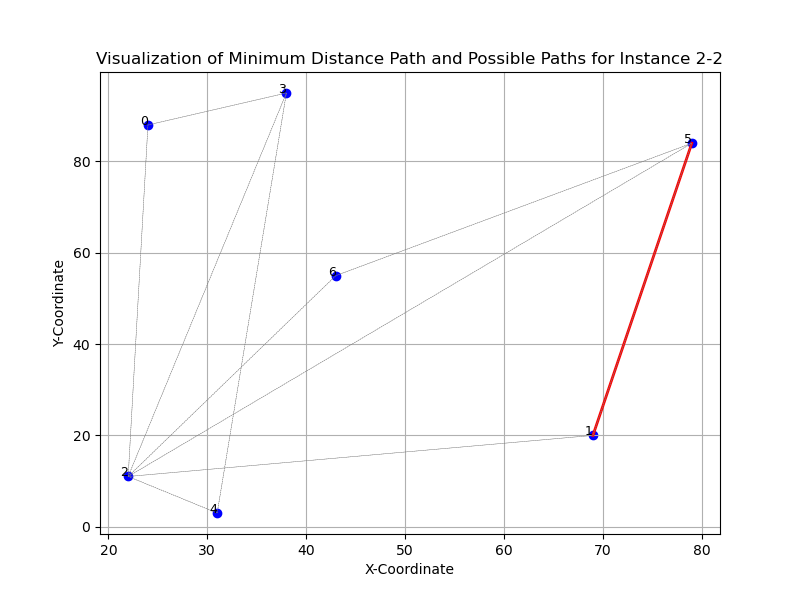
\includegraphics[width=1.1\textwidth]{assets/Img/GraficaCaminoMinimo-2-2.png}
            \caption{Grafo con 7 puntos y conexiones}
      \end{minipage}
      \hfill
      \begin{minipage}{0.49\textwidth}
            \centering
            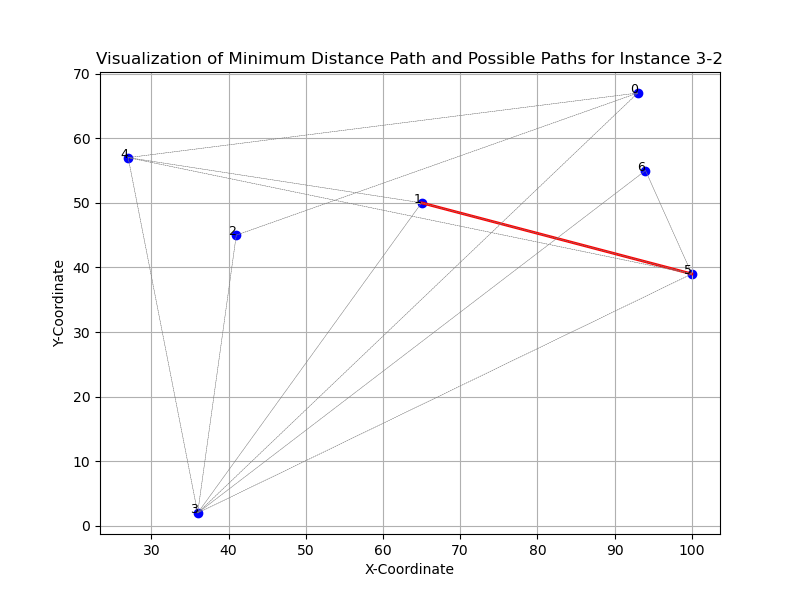
\includegraphics[width=1.1\textwidth]{assets/Img/GraficaCaminoMinimo-3-2.png}
            \caption{Grafo con 7 puntos y conexiones}
      \end{minipage}
\end{figure}
En ambos casos se busca el camino mínimo entre el nodo 1 y 5.\\ \\
Por ultimo expondremos dos ejemplos con 25 puntos en el que se busca el camino mínimo entre el nodo 4 y 11:
\begin{figure}[H]
      \centering
      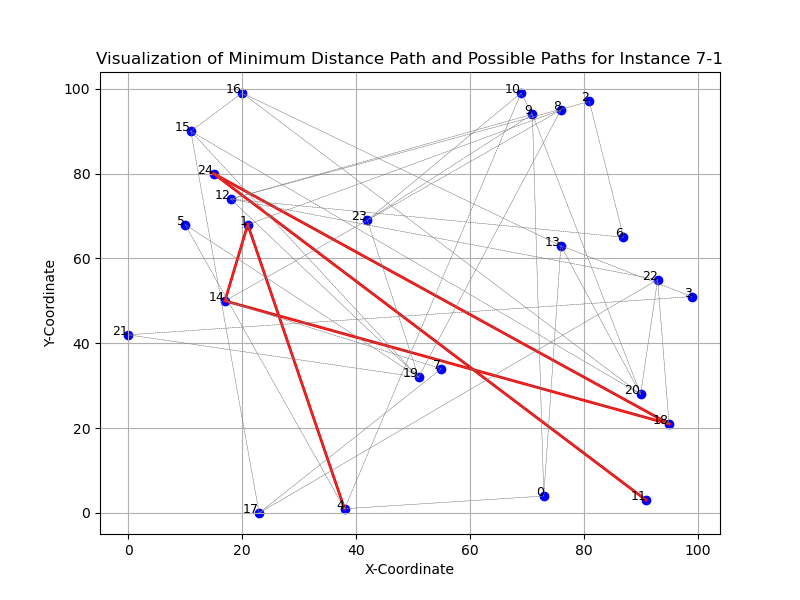
\includegraphics[width=0.65\textwidth]{assets/Img/GraficaCaminoMinimo-7-1.png}
      \caption{Grafo con 25 puntos y conexiones}
      \centering
      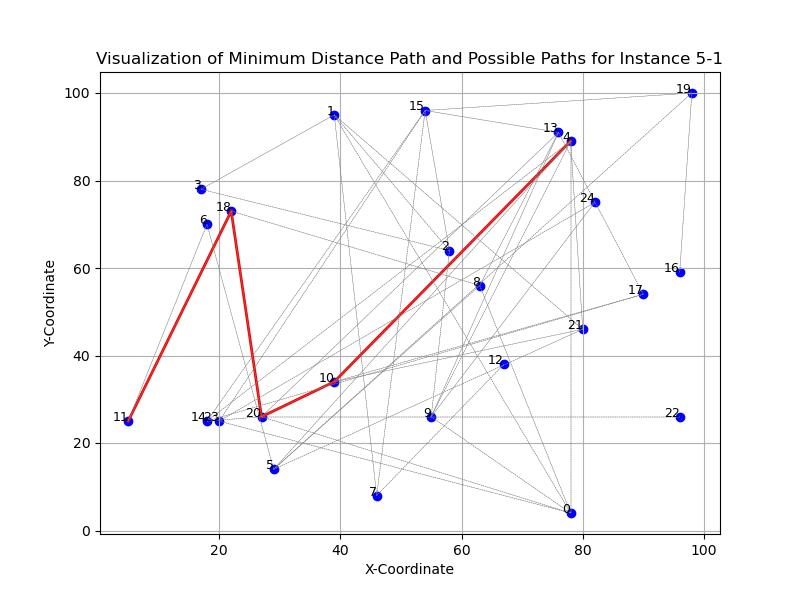
\includegraphics[width=0.65\textwidth]{assets/Img/GraficaCaminoMinimo-5-1.png}
      \caption{Grafo con 25 puntos y conexiones}
\end{figure}
\section{Estudio eficiencia empírica}
% Viajante es el apartado 6, incluir capitulos antes
\chapter{Viajante} % Migue
En esta sección se analiza todo aquello referente al cuarto problema propuesto,
el problema del viajante. Siguiendo las directrices indicadas, se han estudiado
y diseñado diferentes algoritmos "Greedy" que aproximan el problema, con el objetivo
final de comparar cual nos proporciona mejores resultados en cuanto a términos
de eficiencia y precisión. Para determinar esto último, también cabe destacar
detalles de menor importancia como la complejidad de los algoritmos, la estabilidad
frente a distintas entradas o la posibilidad de mejora de los mismos mediante la
elección de distintos puntos de partida o con mejoras posteriores como pueden ser 
aquellas que proporcionan algoritmos como $\lambda$-opt o genéticos.
\\ \\
De aqui en adelante, describiremos por secciones los algoritmos implementados y 
al final proporcionaremos una sección comparativa sobre la cual nos basaremos
para determinar conclusiones, en particular, elegiremos el algoritmo cuya
solución consideremos más conveniente. En lo que sigue se muestra únicamente
el resultado obtenido por el algoritmo sin mejoras posteriores, este tipo de mejoras
suponen una pequeña desvirtuación del objetivo de encontrar el mejor algoritmo y 
es por ello, que su uso se limita a la conclusión final.

\section{Algoritmo \textit{Nearest Neighbour}}
Tal y como el nombre indica, el primer algoritmo implementado no es nada más, ni 
nada menos que el primer algoritmo que probablemente se le puede ocurrir a cualquier
persona que se enfrente a este problema. La idea es sencilla e intuitiva, nos 
dan un conjunto de puntos y queremos encontrar el camino más corto que los recorra,
para ello, \textbf{elegimos} un punto inicial y a partir de ese punto, en un proceso 
iterativo, elegimos en cada paso el siguiente punto más cercano al actual, o lo que 
es lo mismo, el punto para el cual la distancia al punto actual es la menor (No confundir
con el punto para el cual la distancia total es la menor, ya que, aunque parecido, no es 
lo mismo). Este proceso se repite hasta que todos los puntos han sido visitados.
\\ \\
A continuación se proporciona la implementación propuesta del algoritmo en cuestión:
\begin{lstlisting}[language=C++]
vector<Point> nearestNeighborTSP(const vector<Point>& points) {
  vector<Point> path;
  vector<bool> visited(points.size(), false);
  path.reserve(points.size());
  path.emplace_back(points[0]);
  visited[0] = true;

  for (int i = 0; i < points.size() - 1; ++i) {
    double minDistance = numeric_limits<double>::max();
    int nearestNeighbor = -1;
    for (int j = 0; j < points.size(); ++j) {
      if (!visited[j]) {
        double distance = path[i].distanceTo(points[j]);
        if (distance < minDistance) {
          minDistance = distance;
          nearestNeighbor = j;
        }
      }
    }
    path.emplace_back(points[nearestNeighbor]);
    visited[nearestNeighbor] = true;
  }

  return path;
}
\end{lstlisting}
Como se puede apreciar, se ha hecho uso de un vector de puntos visitados (Programación 
dinámica) para evitar visitar un punto más de una vez, esto no supone una complejidad
notable, sin embargo, si que supone una gran mejora en términos de eficiencia. Hemos obviado
un análisis detallado de la eficiencia en este tipo de algoritmos, ya que, en general, resulta
trivial la obtención de la misma, en este caso, claramente estamos ante una eficiencia de
$O(n^2)$.

\section{Algoritmo \textit{Ordenación}}
Como el nombre indica, este algoritmo consiste en ordenar los puntos de partida de
acuerdo a un criterio especifico (en nuestro caso los hemos ordenado por la coordenada
x de menor a mayor, teniendo en cuenta también para puntos cercanos en x, la coordenada y).
Una vez ordenados los puntos, simplemente recorremos el vector de puntos en el orden
en el que se encuentren, de esta forma, el camino total trata de reducir cruces y distancias
con la idea intuitiva de que si dos puntos están cerca en el plano, probablemente, la 
distancia que se recorra al pasar por ellos, sea mínima. Como veremos en el siguiente 
algoritmo y en la conclusión, esto en la práctica no es del todo cierto. Primero veamos 
la implementación del algoritmo:
\begin{lstlisting}[language=C++]
vector<Point> orderedTSP(const vector<Point>& points) {
      vector<Point> tour;
      tour.reserve(points.size());
      copy(points.begin(), points.end(), back_inserter(tour));
      sort(tour.begin(), tour.end());
        
      return tour;
}      
\end{lstlisting}
Como se puede apreciar, la implementación es muy sencilla, simplemente se copian los puntos
de partida a un vector auxiliar, se ordenan y se devuelve el vector ordenado, sin embargo
cuando vemos el resultado de la ejecución, nos damos cuenta de que aunque los puntos
esten muy cerca respecto a la coordenada x, los saltos que se dan en la coordenada y
pueden ser muy grandes, lo que hace que el camino total sea mucho mayor de lo esperado,
además para cerrar el camino, la distancia es la máxima posible en cuanto a x. Para mejorar
esto, podemos observar que si nuestro problema son los saltos en la coordenada y 
y la distancia de cierre, podemos intentar minimizarlos, de donde surge el siguiente
algoritmo. Una vez más, recalcamos que la eficiencia de este algoritmo es $O(n \cdot log(n))$.

\section{Algoritmo \textit{Circular}}
Para solucionar el problema anterior, se propone una alternativa que se basa en la misma
idea de ordenar por la coordenada x, sin embargo, en este caso la coordenada y solo se tiene 
en cuenta tras ordenar, lo que se hace es guardar el la coordenada y de los puntos máximo
y mínimo y se calcula el punto medio entre ambos, esto se hace para recorrer los puntos
de forma circular como el nombre indica, de modo que los puntos que se quedan en la parte 
de abajo del plano, se recorren en sentido horario y los puntos que se quedan en la parte
de arriba del plano, se recorren en sentido antihorario. De esta forma, se consigue minimizar
la cantidad de saltos en el eje y y la distancia de cierre, resulta sugerente pensar que este 
proceso de división en dos partes, se puede hacer de forma recursiva, sin embargo, en la 
práctica, esto supone una complejidad superior a la hora de implementar mas bucles, y no
supone una mejora significativa en términos de precisión, por lo que se ha optado por
dejarlo de esta forma. 
\\ \\
El problema que presenta esta implementación es que dependiendo de la forma que tenga
el conjunto de puntos que se le pase, se obtendrán resultados muy distintos, sin embargo
esto ocurre en todos los algoritmos, por lo que no se considera un problema en si mismo, 
ya que es inherente al problema. A continuación se muestra la implementación del algoritmo:
\begin{lstlisting}[language=C++]
vector<Point> CircTSP(const vector<Point>& points) {
    vector<Point> tour;
    vector<Point> circularTour;
    tour.reserve(points.size());
    circularTour.reserve(points.size());
    tour = points;
    sort(tour.begin(), tour.end());
    
    int min = numeric_limits<int>::max();
    int max = numeric_limits<int>::min();

    for (int i = 0; i < points.size(); ++i) {
        min = min(min, points[i].getY());
        max = max(max, points[i].getY());
    }
    
    double mid = (max + min )/2;

    for (int i = 0; i < points.size(); ++i) {
        if (tour[i].getY() <= mid) {
            circularTour.emplace_back(tour[i]);
        }
    }

    for (int i = points.size(); i >= 0; --i) {
        if (tour[i].getY() > mid) {
            circularTour.emplace_back(tour[i]);
        }
    }

    return circularTour;
}
\end{lstlisting}
Una vez mas, podemos apreciar que se puede aumentar la eficiencia del algoritmo
optimizando bucles y la ordenación de manera que el máximo y el mínimo se calculen
mientras se ordenan los puntos, sin embargo, esto no supone una mejora en cuanto
al orden de eficiencia y si supone una mayor complejidad del codigo, por lo tanto,
como el compilador se encarga de optimizar esos detalles que no afectan al orden
de eficiencia, se ha optado por dejarlo de esta forma para facilitar la lectura, 
en una implementación real, se recomendaría la optimización manual de estos detalles, ya que,
aunque bueno, el compilador no es perfecto y no siempre optimiza de la mejor forma.
Claramente la eficiencia vuelve a ser $O(n \cdot log(n))$.

\section{Algoritmo \textit{SDA}}
El anterior algoritmo, implementa un tipo de solución que quizás podríamos clasificar
más que como \textit{Greedy}, como \textit{Heurística}, por ello, se ha implementado 
un cuarto algoritmo basado en \textit{Greedy}, que aunque no proporciona una solución 
con una idea muy innovadora, entra dentro del tipo de algoritmo requerido. Este algoritmo
es muy parecido a \textit{Nearest Neighbour}, sin embargo, en vez de elegir el punto más
cercano, elige el punto cuya adición al camino total suponga la menor distancia, de primeras
pudiera parecer que estamos haciendo lo mismo, sin embargo, y como confirmaremos más adelante,
esto no es así, ya que el factor distancia de cierre no se tenia en cuenta en el algoritmo
\textit{Nearest Neighbour}. A continuación se muestra la implementación del algoritmo:
\begin{lstlisting}[language=C++]
vector<Point> shortestDistanceTSP(const vector<Point>& points) {
    vector<Point> path;
    vector<bool> visited(points.size(), false);
    path.reserve(points.size());
    path.emplace_back(points[0]);
    visited[0] = true;

    for (int i = 0; i < points.size() - 1; ++i) {
        double minDistance = numeric_limits<double>::max();
        int nearestNeighbor = -1;
        for (int j = 0; j < points.size(); ++j) {
            if (!visited[j]) {
                double distance = path[i].distanceTo(points[j]) + points[j].distanceTo(points[0]);
                if (distance < minDistance) {
                    minDistance = distance;
                    nearestNeighbor = j;
                }
            }
        }
        path.emplace_back(points[nearestNeighbor]);
        visited[nearestNeighbor] = true;
    }

    return path;
}
\end{lstlisting}
Como se puede apreciar, la implementación es muy parecida a la de \textit{Nearest Neighbour},
también, como en todos, la eficiencia se puede mejorar, sin embargo, no supone una mejora
significativa, por lo que se ha optado por dejarlo de esta forma. Para este algoritmo, solo
veremos una parte de la comparativa, ya que, como se ha mencionado, es muy parecido a
\textit{Nearest Neighbour}, y se ha añadido para proporcionar una mayor variedad de algoritmos
y cumplir con el requisito de implementar algoritmos puramente \textit{Greedy}.
Como no podía ser de otra forma, la eficiencia de este algoritmo es $O(n^2)$.


\section{Conclusiones}
Una vez presentados los tres algoritmos, nos disponemos a obtener conclusiones acerca
de ellos así como a compararlos para determinar cual es el mejor, o cómo podríamos
mejorar la precisión de los mismos. Comenzamos mostrando visualmente los resultados
de ejecución de cada uno de ellos, con el objetivo de que el lector pueda apreciar 
de forma sencilla la idea que se ha querido transmitir con cada uno de los algoritmos.
\subsection{Graficas}
% Dos graficas en una fila y una debajo
\begin{figure}[H]
      \centering
      \begin{minipage}{.48\textwidth}
            \centering
            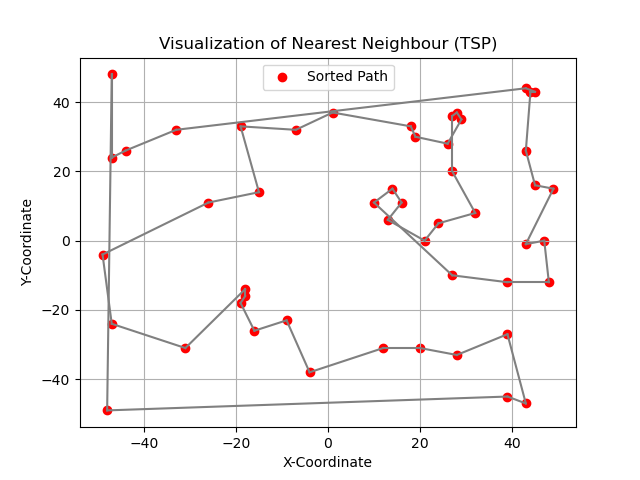
\includegraphics[width=1.1\linewidth]{assets/Img/NearestVisual.png}
            \caption{Nearest Neighbour}
            \label{fig:nearest}
      \end{minipage}%
      \begin{minipage}{.48\textwidth}
            \centering
            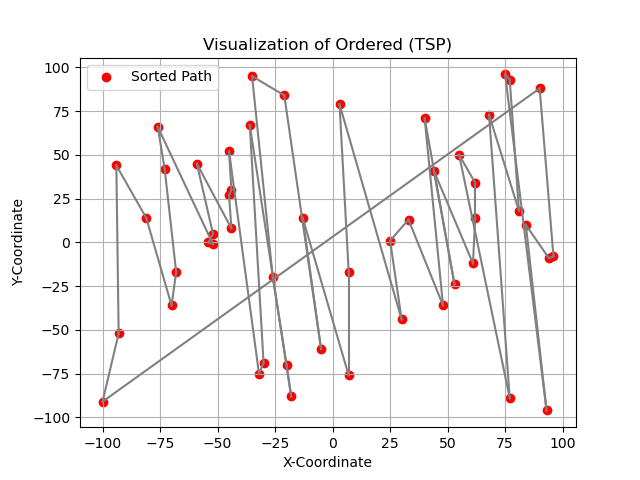
\includegraphics[width=1.1\linewidth]{assets/Img/OrdVisual.png}
            \caption{Ordenación}
            \label{fig:ordered}
      \end{minipage}
\end{figure}
\begin{figure}[H]
      \centering
      \begin{minipage}{.48\textwidth}
            \centering
            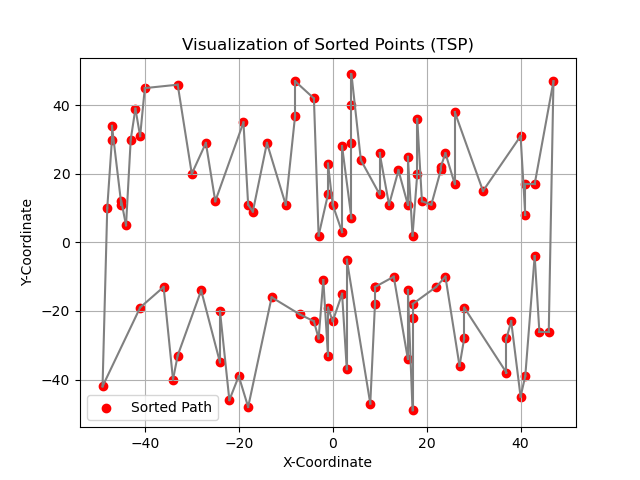
\includegraphics[width=1.1\linewidth]{assets/Img/CircVisual.png}
            \caption{Circular}
            \label{fig:nearest}
      \end{minipage}%
      \begin{minipage}{.48\textwidth}
            \centering
            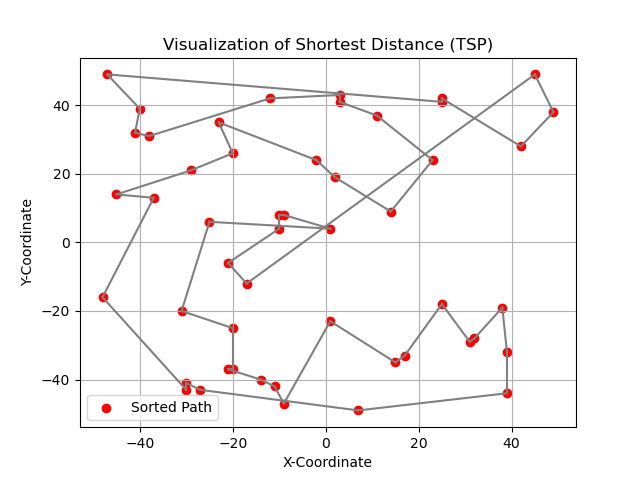
\includegraphics[width=1.1\linewidth]{assets/Img/ShortestVisual.png}
            \caption{Shortest}
            \label{fig:ordered}
      \end{minipage}
\end{figure}
Una vez graficadas, podemos ver los problemas principales de cada uno de los algoritmos,
en el caso de \textit{Nearest Neighbour}, se puede apreciar que la distancia de cierre
es muy grande, sin embargo, aparenta un camino parecido al óptimo, en el caso de 
\textit{Ordenación}, se puede apreciar que, mientras los puntos x están cerca, los saltos
en y son muy grandes, y además la distancia de cierre es máxima, en el caso de \textit{Circular},
se puede apreciar que los saltos en y son más pequeños y la distancia de cierre es menor.
Por último, en el caso de \textit{Shortest}, se puede apreciar el mismo problema que en 
\textit{Nearest Neighbour}, sin embargo, se puede ver que la distancia de cierre tiende a ser
menor.
\\ \\ 
De este análisis visual, podemos deducir que el algoritmo \textit{Nearest Neighbour} es el
que mejor resultado proporciona, obviamente \textit{Shortest Distance} queda muy parecido, a veces
por arriba y otras por abajo, le sigue \textit{Circular} y por último \textit{Ordenación}.
Podríamos dejar el estudio aquí, sin embargo, se proponen maneras de mejorar los algoritmos.
\subsection{Mejoras}
Para mejorar y comparar los algoritmos, comenzamos notando que en el caso de 
\textit{Nearest Neighbour}, la elección del punto de partida nos proporciona un camino
distinto, por lo que, para mejorar la precisión del algoritmo, se puede ejecutar
el algoritmo con distintos puntos de partida y quedarnos con el mejor resultado.
En los casos de \textit{Ordenación} y \textit{Circular}, esto no tendría mucho sentido, 
sin embargo podríamos jugar con la ordenación respecto de un eje u otro, o con la
división en dos partes, respectivamente, para mejorar la precisión de los mismos.
En el caso de \textit{Shortest Distance}, se podría intentar combinar con \textit{Nearest Neighbour}
para obtener un mejor resultado, ya que, como se ha mencionado, es muy parecido a este.
\\ \\
Este tipo de mejoras, son sencillas y no suponen un gran aumento en cuanto al tiempo
de ejecución, sin embargo, tampoco suponen una mejora significativa en cuanto a la
precisión. Su mejor virtud es que nos proporcionan una velocidad de ejecución muy
rápida y una precisión aceptable, por lo que, en la práctica, se recomienda su uso,
sin embargo, habrá aplicaciones en las que se necesite una precisión mayor, en cuyo 
caso se recomienda el uso de algoritmos más complejos como $\lambda$-opt o genéticos.
\subsection{Precisión y Tiempos}
En esta sección se proporcionan los tiempos de ejecución de los algoritmos y se comparan
con la precisión de los mismos, para ello, se han ejecutado los algoritmos sobre un entorno
cuya solución óptima se conoce, de esta forma, se puede comparar la solución obtenida
con la solución óptima, el entorno en cuestión es un conjunto de Paises del mundo
que se han dividido en pueblos y ciudades de interés. A continuación mostramos 
los resultados que hemos obtenido:
\\ \\
Comenzamos exponiendo los resultados que arrojan los algoritmos sin mejoras:
% Dos graficas
\begin{figure}[H]
      \centering
      \begin{minipage}{.48\textwidth}
            \centering
            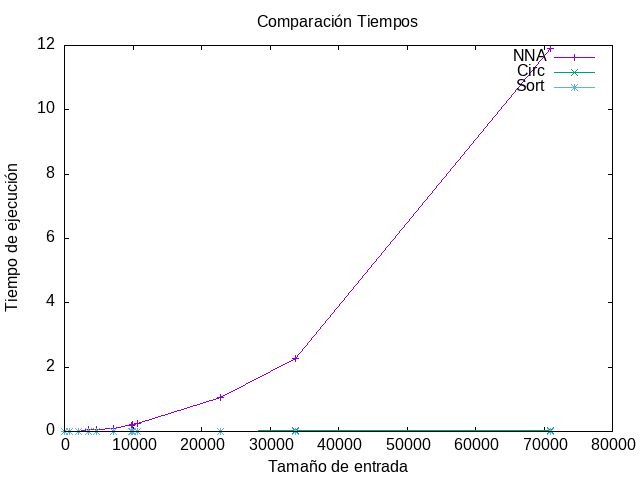
\includegraphics[width=1\linewidth]{assets/Img/Tiempos.png}
            \caption{Tiempos completos}
            \label{fig:nearest}
      \end{minipage}%
      \begin{minipage}{.48\textwidth}
            \centering
            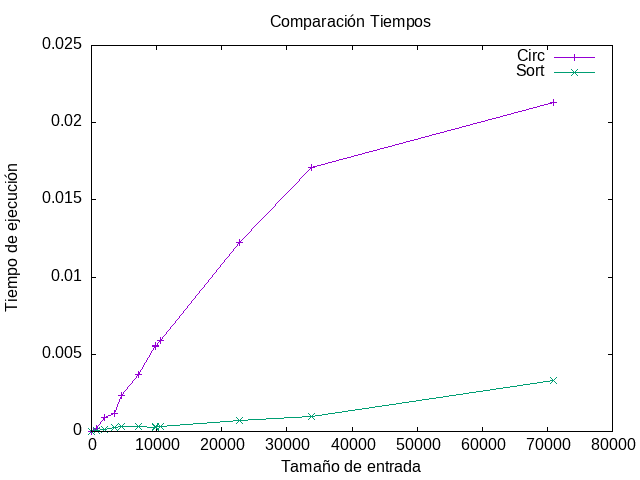
\includegraphics[width=1\linewidth]{assets/Img/TiemposCircSort.png}
            \caption{Tiempos Circ y Sort}
            \label{fig:ordered}
      \end{minipage}
\end{figure}
Como se puede ver, el algoritmo \textit{Nearest Neighbour} es el más lento,
esto era de esperar debido a que, como veremos ahora, es el que mejor precisión
ofrece. El mismo razonamiento se puede aplicar a los algoritmos \textit{Ordenación}
y \textit{Circular}.
Si nos fijamos ahora en los tiempos de ejecución de los algoritmos tras las mejoras,

\begin{figure}[H]
      \centering
      \begin{minipage}{.48\textwidth}
            \centering
            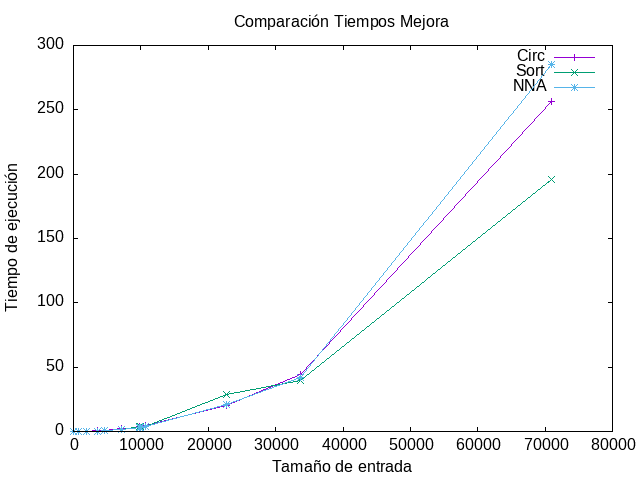
\includegraphics[width=1\linewidth]{assets/Img/TiemposMejora.png}
            \caption{Tiempos completos}
            \label{fig:nearest}
      \end{minipage}%
      \begin{minipage}{.48\textwidth}
            \centering
            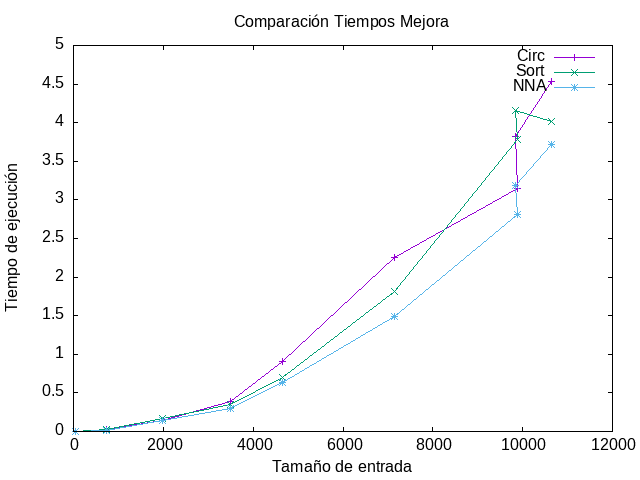
\includegraphics[width=1\linewidth]{assets/Img/TiemposMejoraChico.png}
            \caption{Tiempos menor Tamaño}
            \label{fig:ordered}
      \end{minipage}
\end{figure}
Podemos ver como hay un gran aumento en el tiempo, sin embargo, son tiempos
similares entre ellos, por lo que nos interesa quedarnos con el que mejor precisión
ofrece:
\begin{figure}[H]
      \centering
      \begin{minipage}{.48\textwidth}
            \centering
            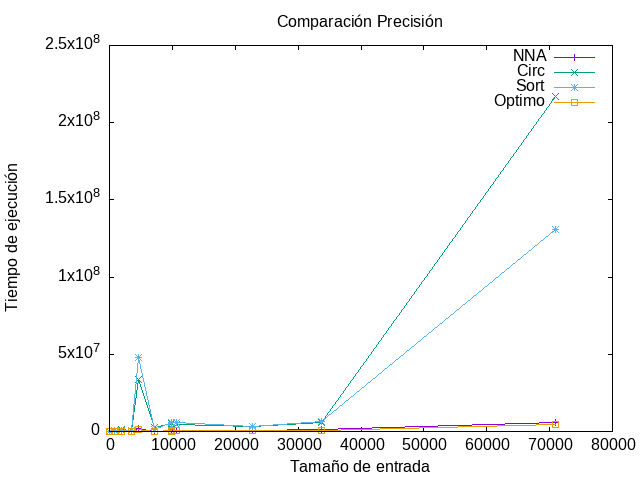
\includegraphics[width=1\linewidth]{assets/Img/Precision.png}
            \caption{Precisión sin mejoras}
            \label{fig:nearest}
      \end{minipage}%
      \begin{minipage}{.48\textwidth}
            \centering
            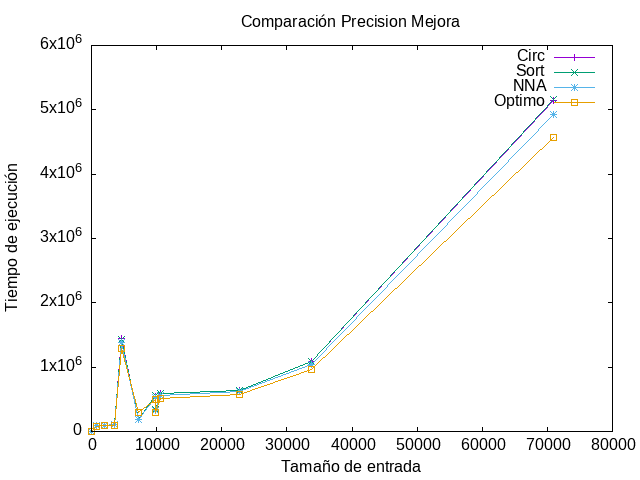
\includegraphics[width=1\linewidth]{assets/Img/PrecisionMejora.png}
            \caption{Precisión tras mejora}
            \label{fig:ordered}
      \end{minipage}
\end{figure}
Como se puede ver, todos los algoritmos con mejora, se quedan muy cerca
de la solución óptima, sin embargo, el algoritmo \textit{Nearest Neighbour}
es el que mejor precisión ofrece, tanto en el caso de mejora como 
en el caso sin mejora, por lo que, en la práctica, se recomienda su uso. Para 
aplicaciones donde la precisión sea un factor crítico, se recomienda el uso
combinado de distintas mejoras como la elección de distintos puntos de partida
o el uso de algoritmos más complejos como $\lambda$-opt o genéticos.

\end{document}